\documentclass[12pt]{report}
\usepackage{scribe,graphicx,graphics}
\usepackage{float}
\usepackage{siunitx}
\usepackage{braket}
\usepackage{listings}
\course{CSE 389D} 	
\coursetitle{Mathematical Modeling}	
\semester{Spring 2025}
\lecturer{} % Due Date: {\bf Mon, Oct 3 2016}}
\lecturetitle{Problem Set}
\lecturenumber{3}   
\lecturedate{}    
\usepackage{enumerate}
\newcommand{\remind}[1]{\textcolor{red}{\textbf{#1}}} %To remind me of unfinished work to fix later
\newcommand{\hide}[1]{} %To hide large blocks of code without using % symbols

\newcommand{\ep}{\varepsilon}
\newcommand{\vp}{\varphi}
\newcommand{\lam}{\lambda}
\newcommand{\Lam}{\Lambda}
%\newcommand{\abs}[1]{\ensuremath{\left\lvert#1\right\rvert}} % This clashes with the physics package
%\newcommand{\norm}[1]{\ensuremath{\left\lVert#1\right\rVert}} % This clashes with the physics package
\newcommand{\floor}[1]{\ensuremath{\left\lfloor#1\right\rfloor}}
\newcommand{\ceil}[1]{\ensuremath{\left\lceil#1\right\rceil}}
\newcommand{\A}{\mathbb{A}}
\newcommand{\B}{\mathbb{B}}
\newcommand{\C}{\mathbb{C}}
\newcommand{\D}{\mathbb{D}}
\newcommand{\E}{\mathbb{E}}
\newcommand{\F}{\mathbb{F}}
\newcommand{\K}{\mathbb{K}}
\newcommand{\N}{\mathbb{N}}
\newcommand{\Q}{\mathbb{Q}}
\newcommand{\R}{\mathbb{R}}
\newcommand{\T}{\mathbb{T}}
\newcommand{\X}{\mathbb{X}}
\newcommand{\Y}{\mathbb{Y}}
\newcommand{\Z}{\mathbb{Z}}
\newcommand{\As}{\mathcal{A}}
\newcommand{\Bs}{\mathcal{B}}
\newcommand{\Cs}{\mathcal{C}}
\newcommand{\Ds}{\mathcal{D}}
\newcommand{\Es}{\mathcal{E}}
\newcommand{\Fs}{\mathcal{F}}
\newcommand{\Gs}{\mathcal{G}}
\newcommand{\Hs}{\mathcal{H}}
\newcommand{\Is}{\mathcal{I}}
\newcommand{\Js}{\mathcal{J}}
\newcommand{\Ks}{\mathcal{K}}
\newcommand{\Ls}{\mathcal{L}}
\newcommand{\Ms}{\mathcal{M}}
\newcommand{\Ns}{\mathcal{N}}
\newcommand{\Os}{\mathcal{O}}
\newcommand{\Ps}{\mathcal{P}}
\newcommand{\Qs}{\mathcal{Q}}
\newcommand{\Rs}{\mathcal{R}}
\newcommand{\Ss}{\mathcal{S}}
\newcommand{\Ts}{\mathcal{T}}
\newcommand{\Us}{\mathcal{U}}
\newcommand{\Vs}{\mathcal{V}}
\newcommand{\Ws}{\mathcal{W}}
\newcommand{\Xs}{\mathcal{X}}
\newcommand{\Ys}{\mathcal{Y}}
\newcommand{\Zs}{\mathcal{Z}}
\newcommand{\ab}{\textbf{a}}
\newcommand{\bb}{\textbf{b}}
\newcommand{\cb}{\textbf{c}}
\newcommand{\db}{\textbf{d}}
\newcommand{\ub}{\textbf{u}}
\newcommand{\sbb}{\textbf{s}}
%\renewcommand{\vb}{\textbf{v}} % This clashes with the physics package (the physics package already defines the \vb command)
\newcommand{\wb}{\textbf{w}}
\newcommand{\xb}{\textbf{x}}
\newcommand{\yb}{\textbf{y}}
\newcommand{\zb}{\textbf{z}}
\newcommand{\vbb}{\textbf{v}}
\newcommand{\Ab}{\textbf{A}}
\newcommand{\Bb}{\textbf{B}}
\newcommand{\Cb}{\textbf{C}}
\newcommand{\Db}{\textbf{D}}
\newcommand{\eb}{\textbf{e}}
\newcommand{\ex}{\textbf{e}_x}
\newcommand{\ey}{\textbf{e}_y}
\newcommand{\ez}{\textbf{e}_z}
\newcommand{\zerob}{\mathbf{0}}
\newcommand{\abar}{\overline{a}}
\newcommand{\bbar}{\overline{b}}
\newcommand{\cbar}{\overline{c}}
\newcommand{\dbar}{\overline{d}}
\newcommand{\ubar}{\overline{u}}
\newcommand{\vbar}{\overline{v}}
\newcommand{\wbar}{\overline{w}}
\newcommand{\xbar}{\overline{x}}
\newcommand{\ybar}{\overline{y}}
\newcommand{\zbar}{\overline{z}}
\newcommand{\Abar}{\overline{A}}
\newcommand{\Bbar}{\overline{B}}
\newcommand{\Cbar}{\overline{C}}
\newcommand{\Dbar}{\overline{D}}
\newcommand{\Ubar}{\overline{U}}
\newcommand{\Vbar}{\overline{V}}
\newcommand{\Wbar}{\overline{W}}
\newcommand{\Xbar}{\overline{X}}
\newcommand{\Ybar}{\overline{Y}}
\newcommand{\Zbar}{\overline{Z}}
\newcommand{\Aint}{A^\circ}
\newcommand{\Bint}{B^\circ}
\newcommand{\limk}{\lim_{k\to\infty}}
\newcommand{\limm}{\lim_{m\to\infty}}
\newcommand{\limn}{\lim_{n\to\infty}}
\newcommand{\limx}[1][a]{\lim_{x\to#1}}
\newcommand{\liminfm}{\liminf_{m\to\infty}}
\newcommand{\limsupm}{\limsup_{m\to\infty}}
\newcommand{\liminfn}{\liminf_{n\to\infty}}
\newcommand{\limsupn}{\limsup_{n\to\infty}}
\newcommand{\sumkn}{\sum_{k=1}^n}
\newcommand{\sumk}[1][1]{\sum_{k=#1}^\infty}
\newcommand{\summ}[1][1]{\sum_{m=#1}^\infty}
\newcommand{\sumn}[1][1]{\sum_{n=#1}^\infty}
\newcommand{\emp}{\varnothing}
\newcommand{\exc}{\backslash}
\newcommand{\sub}{\subseteq}
\newcommand{\sups}{\supseteq}
\newcommand{\capp}{\bigcap}
\newcommand{\cupp}{\bigcup}
\newcommand{\kupp}{\bigsqcup}
\newcommand{\cappkn}{\bigcap_{k=1}^n}
\newcommand{\cuppkn}{\bigcup_{k=1}^n}
\newcommand{\kuppkn}{\bigsqcup_{k=1}^n}
\newcommand{\cappk}[1][1]{\bigcap_{k=#1}^\infty}
\newcommand{\cuppk}[1][1]{\bigcup_{k=#1}^\infty}
\newcommand{\cappm}[1][1]{\bigcap_{m=#1}^\infty}
\newcommand{\cuppm}[1][1]{\bigcup_{m=#1}^\infty}
\newcommand{\cappn}[1][1]{\bigcap_{n=#1}^\infty}
\newcommand{\cuppn}[1][1]{\bigcup_{n=#1}^\infty}
\newcommand{\kuppk}[1][1]{\bigsqcup_{k=#1}^\infty}
\newcommand{\kuppm}[1][1]{\bigsqcup_{m=#1}^\infty}
\newcommand{\kuppn}[1][1]{\bigsqcup_{n=#1}^\infty}
\newcommand{\cappa}{\bigcap_{\alpha\in I}}
\newcommand{\cuppa}{\bigcup_{\alpha\in I}}
\newcommand{\kuppa}{\bigsqcup_{\alpha\in I}}
\newcommand{\Rx}{\overline{\mathbb{R}}}
\newcommand{\dx}{\,dx}
\newcommand{\dy}{\,dy}
\newcommand{\dt}{\,dt}
\newcommand{\dax}{\,d\alpha(x)}
\newcommand{\dbx}{\,d\beta(x)}
\DeclareMathOperator{\glb}{\text{glb}}
\DeclareMathOperator{\lub}{\text{lub}}
\newcommand{\xh}{\widehat{x}}
\newcommand{\yh}{\widehat{y}}
\newcommand{\zh}{\widehat{z}}
\newcommand{\<}{\langle}
\renewcommand{\>}{\rangle}
\renewcommand{\iff}{\Leftrightarrow}
\DeclareMathOperator{\im}{\text{im}}
\let\spn\relax\let\Re\relax\let\Im\relax
\DeclareMathOperator{\spn}{\text{span}}
\DeclareMathOperator{\sym}{\text{Sym}}
\DeclareMathOperator{\myskew}{\text{Skew}}
\DeclareMathOperator{\Re}{\text{Re}}
\DeclareMathOperator{\Im}{\text{Im}}
\DeclareMathOperator{\diag}{\text{diag}}
\endinput
\usepackage{xcolor}

\definecolor{codegreen}{rgb}{0,0.6,0}
\definecolor{codegray}{rgb}{0.5,0.5,0.5}
\definecolor{codepurple}{rgb}{0.58,0,0.82}
\definecolor{backcolour}{rgb}{0.95,0.95,0.92}

\lstdefinestyle{mystyle}{
    backgroundcolor=\color{backcolour},   
    commentstyle=\color{codegreen},
    keywordstyle=\color{magenta},
    numberstyle=\tiny\color{codegray},
    stringstyle=\color{codepurple},
    basicstyle=\ttfamily\footnotesize,
    breakatwhitespace=false,         
    breaklines=true,                 
    captionpos=b,                    
    keepspaces=true,                 
    numbers=left,                    
    numbersep=5pt,                  
    showspaces=false,                
    showstringspaces=false,
    showtabs=false,                  
    tabsize=2
}

\lstset{style=mystyle}
\theoremheaderfont{\itshape}
\theorembodyfont{\upshape}
\newtheorem{case}{Case}

% Insert your name here!
\scribe{Student Name: Noah Reef}
\newcommand{\rb}{\bold{r}}

\begin{document}
\maketitle
\section*{Problem 3.1}
\subsection*{Part a}
Recall that the angular momentum operator of a particle is given by
\begin{align*}
  \hat{L} = \hat{r} \times \hat{p} = (\hat{r}_y \hat{p}_z - \hat{r}_z \hat{p}_y) u_x + (\hat{r}_z \hat{p}_x - \hat{r}_x \hat{p}_z) u_y + (\hat{r}_x \hat{p}_y - \hat{r}_y \hat{p}_x) u_z
\end{align*}
then we have that 
\begin{align*}
  [\hat{L}_x, \hat{L}_y] &= [\hat{r}_y \hat{p}_z - \hat{r}_z \hat{p}_y, \hat{r}_z \hat{p}_x - \hat{r}_x \hat{p}_z] \\ 
                         &= [\hat{r}_y\hat{p}_z, \hat{r}_z\hat{p}_x] - [\hat{r}_y\hat{p}_z, \hat{r}_x\hat{p}_z] - [\hat{r}_z\hat{p}_y, \hat{r}_z\hat{p}_x] + [\hat{r}_z\hat{p}_y, \hat{r}_x\hat{p}_z] \\
                         &= [\hat{r}_y\hat{p}_z,\hat{r_z}] \hat{p}_x + \hat{r}_z[\hat{r}_y\hat{p}_z,\hat{p}_x] - [\hat{r}_y\hat{p}_z,\hat{r}_x]\hat{p}_z \\
                         &- \hat{r}_x[\hat{r}_y\hat{p}_z,\hat{p}_z] - [\hat{r}_z\hat{p}_y,\hat{r}_z]\hat{p}_x - \hat{r}_z[\hat{r}_z\hat{p}_y,\hat{p}_x] + [\hat{r}_z\hat{p}_y,\hat{r}_x]\hat{p}_z + \hat{r}_x[\hat{r}_z\hat{p}_y,\hat{p}_z] \\
\end{align*}
then we see that
\begin{align*}
  [\hat{r}_y\hat{p}_z, \hat{r}_z] &= \hat{r}_y[\hat{p}_z,\hat{r}_z] + [\hat{r}_y,\hat{r}_z]\hat{p}_z = -i\hbar \hat{r}_y \\
  [\hat{r}_y\hat{p}_z, \hat{p}_x] &= \hat{r}_y[\hat{p}_z, \hat{p}_x] + [\at{r}_y, \hat{p}_x] \hat{p}_y = 0 \\
  [\hat{r}_y\hat{p}_z, \hat{r}_x] &= 0 \\
  [\hat{r}_y\hat{p}_z, \hat{p}_z] &= 0 \\
  [\hat{r}_z \hat{p}_y, \hat{r}_z] &= 0 \\
  [\hat{r}_z \hat{p}_y, \hat{p}_x] &= 0 \\
  [\hat{r}_z \hat{p}_y, \hat{r}_x] &= 0 \\
  [\hat{r}_z \hat{p}_y, \hat{p}_z] &= i\hbar \hat{p}_y
  \end{align*}
  and hence 
  \begin{equation*}
    [\hat{L}_x, \hat{L}_y] = -i\hbar \hat{r}_y \hat{p}_x + i\hbar \hat{r}_x \hat{p}_y = i\hbar \hat{L}_z
  \end{equation*}
  as desired.

  \subsection*{Part b}
  We have that 
  \begin{align*}
    [\hat{L}_z, \hat{L}^2] &= [\hat{L}_z, \hat{L}_x^2 + \hat{L}_y^2 + \hat{L}_z^2] = [\hat{L}_z, \hat{L}_x^2] + [\hat{L}_z, \hat{L}_y^2] + [\hat{L}_z, \hat{L}_z^2] \\
    &= [\hat{L}_z, \hat{L}_x]\hat{L}_x + \hat{L}_x[\hat{L}_z, \hat{L}_x] + [\hat{L}_z, \hat{L}_y]\hat{L}_y + \hat{L}_y[\hat{L}_z, \hat{L}_y] + [\hat{L}_z, \hat{L}_z]\hat{L}_z + \hat{L}_z[\hat{L}_z, \hat{L}_z]\\
    &= 2i\hbar \hat{L}_x\hat{L}_y- 2i\hbar \hat{L}_y \hat{L}_x = 0
  \end{align*}

  \subsection*{Part c}
  Suppose that $\ket{\epsilon}$ is an eigenstate of $\hat{L}_z$, then we have that 
  \begin{equation*}
    \hat{L}_z\ket{\epsilon} = \epsilon\ket{\epsilon}
  \end{equation*}
  and notice that from part b, we showed that $[\hat{L}_z, \hat{L}^2] = 0$ and hence we have that
  \begin{equation*}
    \hat{L}^2 \hat{L}_z \ket{\epsilon} = \epsilon \hat{L}^2 \ket{\epsilon} =  \hat{L}_z \hat{L}^2 \ket{\epsilon}
  \end{equation*}
  an hence $\hat{L}^2 \ket{\epsilon} = K \ket{\epsilon}$ and hence $\ket{\epsilon}$ is also an eigenstate of $\hat{L}^2$.


\section*{Problem 3.2}
\subsection*{Part a}
Suppose we have the Hamilton operator of a certain quantum system in Dirac's notation
\begin{equation*}
  \hat{H} = E_0 = \sum_{n=1}^\infty n^2 \ket{n}\bra{n}
\end{equation*}
then we see that
\begin{align*}
  \hat{H} \ket{m} &= E_0 \sum_{n=1}^\infty n^2 \ket{n}\bra{n}\ket{m} \\
    &= E_0 \sum_{n=1}^\infty n^2 \ket{n}\delta_{nm} \\
    &= E_0 m^2 \ket{m}
\end{align*}
thus $\ket{m}$ is an eigenstate of $\hat{H}$ with eigenvalue $E_0 m^2$, where $m$ is a positive integer.

\subsection*{Part b}
We can define a square root operator of $\hat{H}$ as 
\begin{equation*}
  \hat{H}^{1/2} = \sqrt{E_0} \sum_{n=1}^\infty n \ket{n}\bra{n}
\end{equation*}
since each of the $\ket{n}$ are orthogonal, we have that each of the off-diagonal terms are zero and hence we are left with the diagonal terms and hence get the form above. 

\subsection*{Part c}
Note that using the form of $\hat{H}^{1/2}$ above, we can see that
\begin{equation*}
  \hat{H}^{1/2} = \sqrt{E_0} \sum_{n=1}^\infty (-1)^{mn}n \ket{n}\bra{n}
\end{equation*}
for any choice $m \in \mathbb{Z}$, are also square-root operators of $\hat{H}$, and thus there are infinitely many square-root operators of $\hat{H}$.

\subsection*{Part d}
Looking at the eigenvalue spectrum of the Hamiltonian in part a, we see that this system describes a particle in the one-dimensional infinite square well potential
\begin{equation*}
  V(x) = \begin{cases}
    -V_0 & |x| < a \\
    \infty & |x| > a
  \end{cases}
\end{equation*}
the square-root operator, $\hat{H}$, is associated with the magnitude of the momentum of the particle.

\section*{Problem 3.3}
\subsection*{Part a}
Suppose that we have the one-dimensional quartic anharmonic oscillator
\begin{equation*}
  \hat{H} = \frac{\hat{p}^2}{2m} + \frac{1}{2}m\omega^2 \hat{x}^2 + \kappa \frac{m^2 \omega^3}{\hbar} \hat{x}^4
\end{equation*}
recall that 
\begin{align*}
  \hat{a} &= \sqrt{\frac{m\omega}{2\hbar}}\left(\hat{x} + i \frac{\hat{p}}{m\omega}\right) \\
  \hat{a}^\dagger &= \sqrt{\frac{m\omega}{2\hbar}}\left(\hat{x} - i \frac{\hat{p}}{m\omega}\right)
\end{align*}
and we compute that
\begin{align*}
\hat{a}^\dagger \hat{a} &= \frac{m \omega}{2\hbar}\left(\hat{x} - i \frac{\hat{p}}{m\omega}\right)\left(\hat{x} + i \frac{\hat{p}}{m\omega}\right) \\
                        &= \frac{m \omega}{2\hbar}\left(\hat{x}^2 + i\frac{\hat{x} \hat{p}}{m\omega} - i \frac{\hat{p}{\hat{x}}}{m \omega} + \frac{\hat{p}^2}{m^2 \omega^2}\right) \\
                        &= \frac{m\omega}{2\hbar} \left(\hat{x}^2 + i \frac{[\hat{x},\hat{p}]}{m\omega} + \frac{\hat{p}^2}{m^2 \omega^2}\right) \\
                        &= \frac{m\omega}{2\hbar} \left(\hat{x}^2 - \frac{\hbar}{m\omega} + \frac{\hat{p}^2}{m^2 \omega^2}\right) \\
                        &= -\frac{1}{2} + \frac{m \omega}{2\hbar} \hat{x}^2 + \frac{\hat{p}^2}{2\hbar m\omega}
\end{align*}
and
\begin{align*}
  \hat{a} + \hat{a}^\dagger = \sqrt{\frac{m \omega}{2\hbar}} 2\hat{x}
\end{align*}
then we see that
\begin{align*}
  \frac{1}{2} + \hat{a}^\dagger \hat{a} + \frac{\kappa}{4}(\hat{a} + \hat{a}^\dagger)^4 &=  \frac{1}{2} + \left(-\frac{1}{2} + \frac{m \omega}{2\hbar} \hat{x}^2 + \frac{\hat{p}^2}{2\hbar m\omega}\right) + \frac{\kappa}{4}\left( \frac{4 m^2 \omega^2}{\hbar^2} \hat{x}^4 \right) \\
                                                                                        &= \left(\frac{m\omega}{2\hbar} \hat{x}^2 + \frac{\hat{p}}{2\hbar m \omega} + \frac{\kappa m^2 \omega^2}{\hbar^2} \hat{x}^4\right) \\
                                                                                        &= \frac{1}{\hbar \omega} \left(\frac{m\omega^2}{2} \hat{x}^2 + \frac{\hat{p}}{2m} + \kappa \frac{m^2 \omega^3}{\hbar} \hat{x}^4\right) \\
                                                                                        &= \frac{\hat{H}}{\hbar \omega} 
\end{align*}

\subsection*{Part b}
Consider 
\begin{align*}
  (\hat{a} + \hat{a}^\dagger)^4 &=(\hat{a} + \hat{a}^\dagger)^2(\hat{a} + \hat{a}^\dagger)^2 
\end{align*}
Then for
\begin{align*}
  (\hat{a} + \hat{a}^\dagger)^2 &= (\hat{a}^2 + \hat{a}\hat{a}^\dagger + \hat{a}^\dagger \hat{a} + \hat{a}^{\dagger^2}) \\
                                &= (\hat{a}^2 + 1 + 2\hat{a}^\dagger \hat{a} + \hat{a}^{\dagger^2}) \\
                                &= (\hat{a}^2 + 1 + 2 \hat{N}+ \hat{a}^{\dagger^2}) 
\end{align*}
thus
\begin{equation*}
  (\hat{a} + \hat{a}^\dagger)^4 = (\hat{a}^2 + \hat{a}^{\dagger^2})^2 + (\hat{a}^2 + \hat{a}^{\dagger^2})(1 + 2\hat{N}) + (1 + 2\hat{N})(\hat{a}^2 + \hat{a}^{\dagger^2}) + (1 + 2\hat{N})^2
\end{equation*}
and we have that
\begin{align*}
  (\hat{a}^2 + \hat{a}^{\dagger^2}) &= \hat{a}^4 + \hat{a}^2 \hat{a}^{\dagger^2} + \hat{a}^{\dagger^2}\hat{a}^2 + \hat{a}^{\dagger^2} \\
  (\hat{a}^2 + \hat{a}^{\dagger^2})(1 + 2\hat{N}) &= \hat{a}^2 + 2\hat{a}^2\hat{N} + \hat{a}^{\dagger^2} + 2\hat{a}^{\dagger^2}\hat{N}\\
  (1 + 2\hat{N})(\hat{a}^2 + \hat{a}^{\dagger^2}) &= \hat{a}^2 + 2\hat{N}\hat{a}^2 + \hat{a}^{\dagger^2} + 2\hat{N}\hat{a}^{\dagger^2}\\
  (1 + 2\hat{N})^2 &= 1 + 4\hat{N} + 4\hat{N}^2
\end{align*}
and hence
\begin{equation*}
  (\hat{a} + \hat{a}^\dagger)^4 = \hat{a}^4 + \hat{a}^{\dagger^2} + 2 (\hat{a}^2 + \hat{a}^{\dagger^2}) + 2\left[\hat{N}(\hat{a}^2 + \hat{a}^{\dagger^2}) + (\hat{a}^2 + \hat{a}^{\dagger^2})\hat{N}\right] + \hat{a}^2\hat{a}^{\dagger^2} + \hat{a}^{\dagger^2}\hat{a}^2 + 4\hat{N} + 4\hat{N}^2 + 1
\end{equation*}
then we have
\begin{align*}
  \hat{a}^2 \hat{a}^{\dagger^2} &= 2 + 3\hat{N} + \hat{N}^2 \\
  \hat{a}^{\dagger^2} \hat{a}^2 &= \hat{N}^2 - \hat{N} \\
\end{align*}
and so we have that
\begin{equation*}
  (\hat{a} + \hat{a}^\dagger)^4 =\hat{a}^4 + \hat{a}^{\dagger^4} + 2 (\hat{a}^2 + \hat{a}^{\dagger^2}) + 2\left[\hat{N}(\hat{a}^2 + \hat{a}^{\dagger^2}) + (\hat{a}^2 + \hat{a}^{\dagger^2})\hat{N}\right] + 3 + 6\hat{N} + 6\hat{N}^2
\end{equation*}

\subsection*{Part c}
Let $\kappa = 0$, and let $\ket{n}$ be an eigenstate of $\hat{H}$, then we have that
\begin{equation*}
  \hat{a} \ket{n} = \sqrt{n} \ket{n-1} \implies \hat{a}^2 \ket{n} = \sqrt{n(n-1)} \ket{n-2}
\end{equation*}
and thus
\begin{equation*}
  \bra{n}\hat{a}^2\ket{n} = \sqrt{n(n-1)} \braket{n|n-2} = 0
\end{equation*}
since $\ket{n}$ and $\ket{n-2}$ are orthogonal. Now we consider,
\begin{equation*}
  \hat{a}^\dagger \ket{n} = \sqrt{n+1} \ket{n+1} \implies \hat{a}^{\dagger^2} \ket{n} = \sqrt{(n+1)(n+2)} \ket{n+2}
\end{equation*}
then we have that
\begin{equation*}
  \bra{n}\hat{a}^{\dagger^2}\ket{n} = \sqrt{(n+1)(n+2)} \braket{n|n+2} = 0
\end{equation*}
since $\ket{n}$ and $\ket{n+2}$ are orthogonal. Lastly we have that
\begin{align*}
  \bra{n}\hat{a}^4\ket{n} &= \sqrt{n(n-1)(n-2)(n-3)} \braket{n|n-4} = 0 \\
  \bra{n}\hat{a}^{\dagger^4}\ket{n} &= \sqrt{(n+1)(n+2)(n+3)(n+4)} \braket{n|n+4} = 0
\end{align*}

\subsection*{Part d}
\begin{align*}
  \bra{n}\hat{N}\hat{a}^2 \ket{n} &= \sqrt{n(n-1)} \bra{n}\hat{N}\ket{n-2} = (n-2)\sqrt{n(n-1)} \braket{n|n-2} = 0\\
\bra{n}\hat{N}\hat{a}^{\dagger^2} \ket{n} &= \sqrt{(n+1)(n+2)} \bra{n}\hat{N}\ket{n+2} = (n+2)\sqrt{(n+1)(n+2)}\braket{n|n+2} = 0 \\
\bra{n} \hat{a}^2 \hat{N} \ket{a} &= n \bra{n}\hat{a}^2 \ket{n} = n\sqrt{n(n-1)} \braket{n|n-2} = 0 \\
\bra{n} \hat{a}^{\dagger^2} \hat{N} \ket{a} &= n \bra{n}\hat{a}^{\dagger^2} \ket{n} = n\sqrt{(n+1)(n+2)} \braket{n|n+2} = 0
\end{align*}

\subsection*{Part e}
\begin{equation*}
  \bra{n}\hat{H} \ket{n} = \hbar \omega \left(\frac{1}{2} \braket{n|n} + \bra{n}\hat{N}\ket{n} + \frac{\kappa}{4} \bra{n}(\hat{a} + \hat{a}^\dagger)^4 \ket{n}\right)
\end{equation*}
note that
\begin{align*}
  \braket{n|n} &= 1 \\
  \bra{n} \hat{N} \ket{n} &= n \braket{n|n} = n \\
  \bra{n} (\hat{a} + \hat{a}^\dagger) \ket{n} &= \bra{n}\hat{a}^4 + \hat{a}^{\dagger^4} + 2 (\hat{a}^2 + \hat{a}^{\dagger^2}) + 2\left[\hat{N}(\hat{a}^2 + \hat{a}^{\dagger^2}) + (\hat{a}^2 + \hat{a}^{\dagger^2})\hat{N}\right] + 3 + 6\hat{N} + 6\hat{N}^2 \ket{n} 
\end{align*}
and we have that the above reduces to
\begin{equation*}
  \bra{n} (\hat{a} + \hat{a}^\dagger) \ket{n} = 3 \braket{n|n} + 6\bra{n}\hat{N}\ket{n} + 6\bra{n}\hat{N}^2\ket{n} = 3 + 6n + 6n^2
\end{equation*}
and hence
\begin{equation*}
  \bra{n} \hat{H} \ket{n} = \hbar\omega \left(\frac{1}{2} + n\right) + \frac{\kappa \hbar \omega}{4} \left(2 + 6n + 6n^2\right)
\end{equation*}

\subsection*{Part f \& g}
\begin{figure}[H]
  \centering
  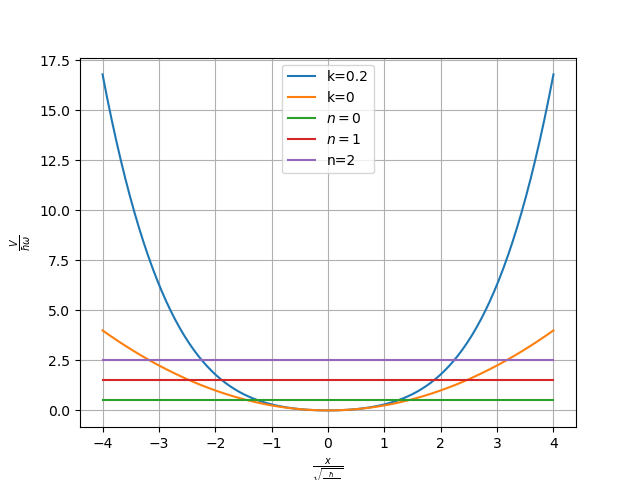
\includegraphics[scale=0.8]{hw3q3f.png}
  \caption{$\frac{V}{\hbar \omega}$ vs $x/(\sqrt{\hbar/2m\omega})$}
\end{figure}
\end{document}

